\documentclass[10pt]{standalone}
\usepackage{amsmath}
\usepackage{pgf,tikz}
\usetikzlibrary{calc}
\usepackage{mathrsfs}
\usetikzlibrary{arrows}
\pagestyle{empty}
\begin{document}
	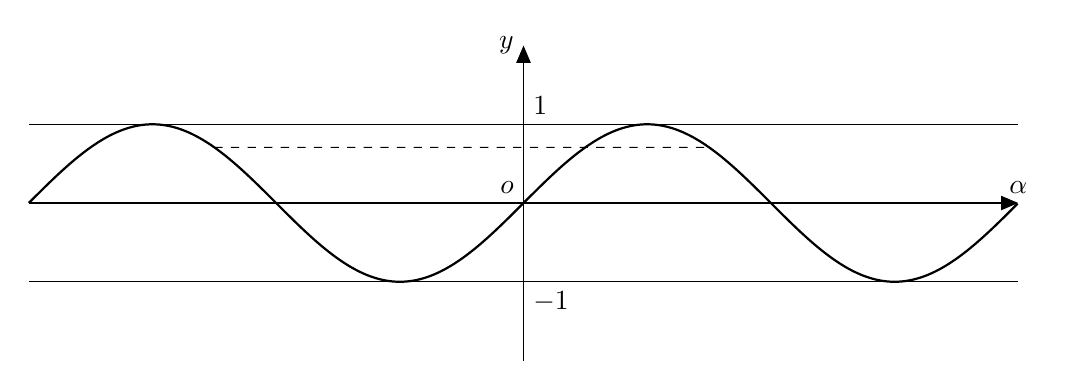
\begin{tikzpicture}[>=triangle  45]
	\tikzset{samples=600}
	\pgfmathsetmacro{\a}{1};
	\pgfmathsetmacro{\Xm}{-2*pi};
	\pgfmathsetmacro{\XM}{2*pi};
	\coordinate [label=above left:$o$] (oo)  at (0,0);
	\coordinate (A) at (-5/4*pi,{\a*sin(-5/4*pi r)});
	\coordinate (B) at (3/4*pi,{\a*sin(3/4*pi r)});
	\node (C )at (0,\a)[above right] {$1$};
	\node (D )at (0,-\a)[below right] {$-1$};
	\draw[->] (\Xm,0) -- (\XM,0) node[above] {$\alpha$} ;
	\draw[->] (0,-\a-1) -- (0,\a+1) node[left] {$y$} ;
	\draw (\Xm,\a) -- (\XM,\a) ;
	\draw (\Xm,-\a) -- (\XM,-\a) ;
	\draw [thick, domain=\Xm:\XM] plot  (\x,{\a*sin(\x r)});  
	\draw[dashed] (A)-- (B) ;  
	\end{tikzpicture}
\end{document}